\section{Indium Electroplating}

\subsection{Introduction}
There are a variety of methods for indium electroplating, while I did not select the electroplating process there are a variety of methods available that are commonly used in industry. The largest differences tend to be in what comprises the solution and the operating temperatures.

\subsection{Process}
The indium electroplating process is based on a now industry standard process that is known to yield good results while requiring a minimum of process optimization. Indium easily allows for wafer bumping where the deformability, low melting point, and cold welding properties \cite{indiumCorpPulsing}. While other alloys consisting of tin and lead or tin, silver, and copper are also used for these processes they come with other disadvantages such as large crystal sizes and high sensitivity to temperature. The plating solution provided by Indium corporation contains


Adapting the indium electroplating process to the E3-3139 and the resources available there, the process is in \hyperref[sec:SOP]{Appendix A}.

The process used there allows us to electroplate indium onto the substrate that is Chrome-Gold on Sapphire. Gold is an excellent material for indium to easily electroplate onto, and is particularly effective for eutectic bonding for $\ch{In}-\ch{Au}$ as the alloy that is formed is able to effectively join the wafers \cite{waferBondingHandbook}.

\begin{figure}[b!]
    \centering
    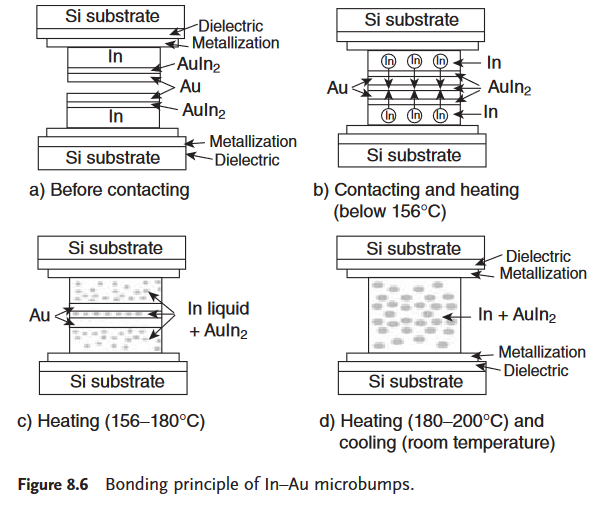
\includegraphics[width=0.6\textwidth]{Main/Ch1/indium_bonding.png}
    \caption{\raggedright Eutectic bonding of $\ch{In}-\ch{Au}$ micro-bumps}
\end{figure}


\newpage

\subsection{Existing Setup Description}

In summary the process has us prepare the sample with acids before placing into the plating solution. Then the sample holder and sample are submerged in the plating solution and the current source is applied. However, due to cost constraints a voltage source was obtained to perform in place of a current source.

\begin{wrapfigure}{L}{0.25\textwidth}
    \centering
    \includegraphics[width=0.25\textwidth, angle=90]{Main/Ch1/Aligator_clip.jpeg}
    \caption{\raggedright Image of the flat mouth alligator clip used to clamp onto the sample}
\end{wrapfigure}

A current source would have been preferred over a voltage source due to several reasons. Since electroplating is a process where metal ions are deposited on a substrate through the use of an electric current. The amount of metal deposited is directly proportional to the amount of electric charge that flows through the system, which means that controlling the current is crucial for controlling the thickness and quality of the plated layer.

With a current source, the current can be precisely controlled and maintained at a constant level, which results in consistent and uniform plating as a function of time. On the other hand, a voltage source may not provide a consistent current, as the resistance of the plating solution can vary due to factors such as temperature or impurities, leading to poor plating results.

\begin{wrapfigure}{R}{0.25\textwidth}
    \centering
    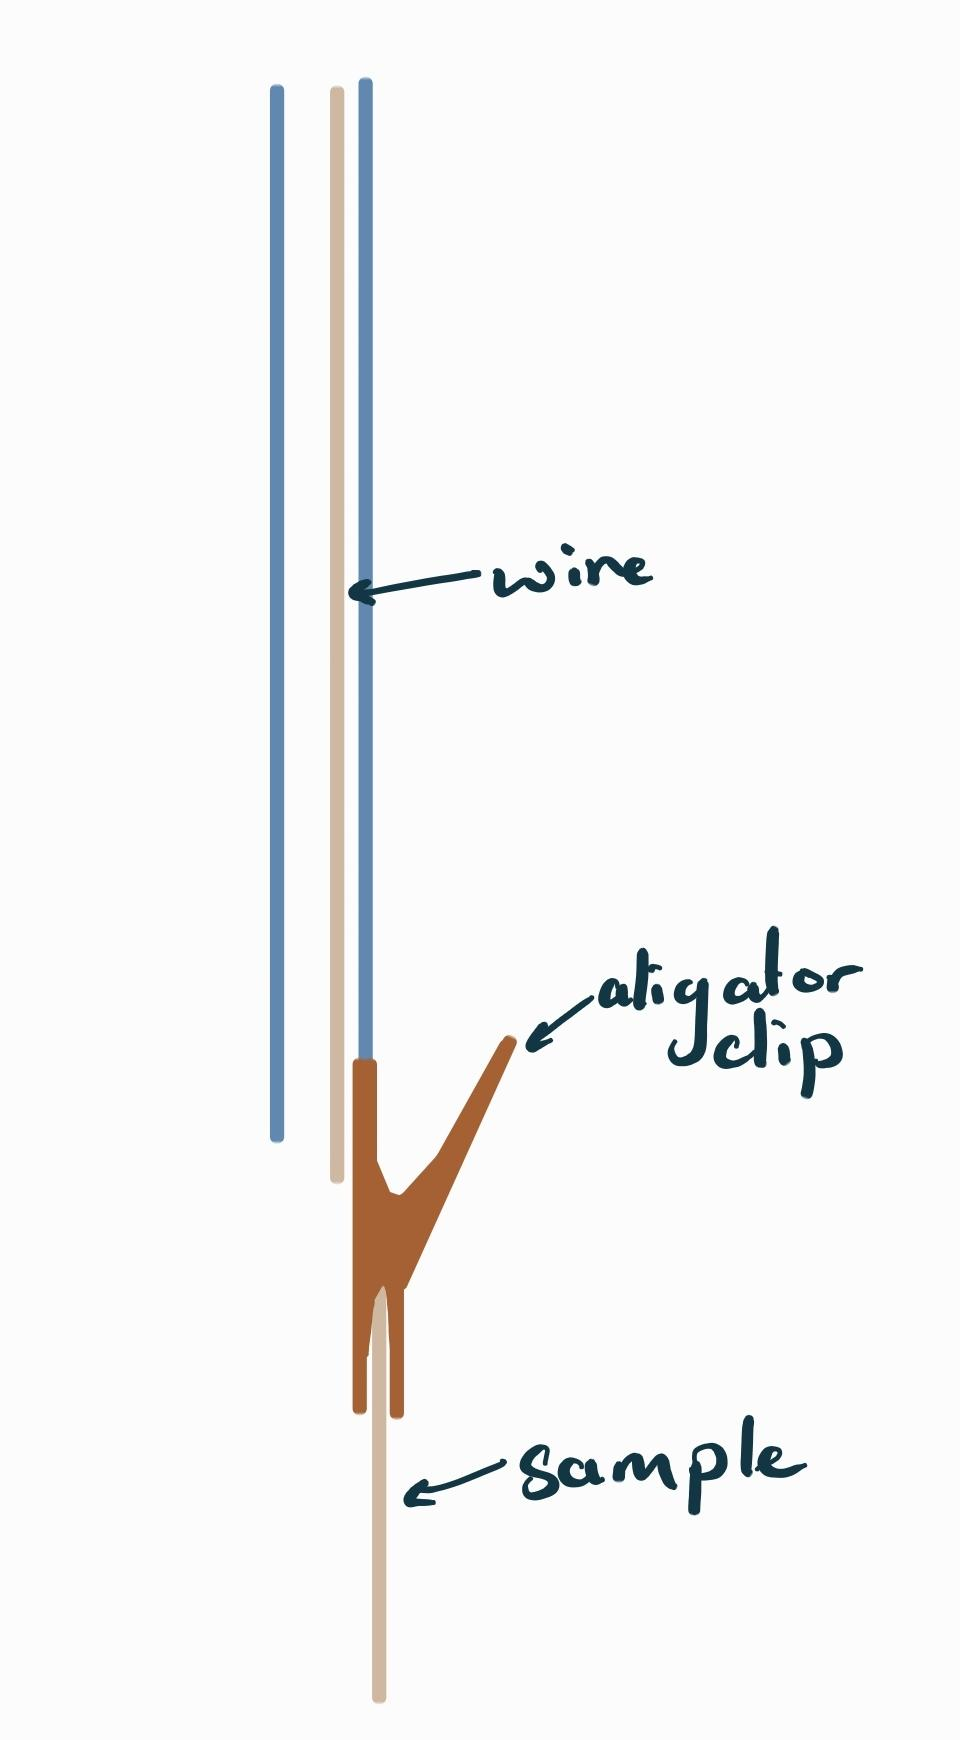
\includegraphics[width=0.25\textwidth]{Main/Ch1/Current Sample holder.png}
    \caption{Line drawing of the alligator clip and sample }
\end{wrapfigure}

Another advantage of using a current source is that it allows for better control over the plating process and reduces the risk of over-plating or under-plating. With a voltage source, the voltage applied to the system can cause the plating rate to fluctuate, which can result in uneven thickness or even damage to the substrate. In contrast, a current source ensures a constant and controlled deposition rate, which minimizes the risk of defects or damage to the substrate.

Using a voltage source with an ammeter can be equivalent to a current source in certain situations. This is because the voltage applied to a circuit is directly proportional to the current flowing through it. By measuring the current in the circuit using an ammeter, the current can be controlled by adjusting the voltage. In this way, the voltage source with an ammeter can effectively act as a current source.


\begin{wrapfigure}{L}{0.25\textwidth}
    \centering
    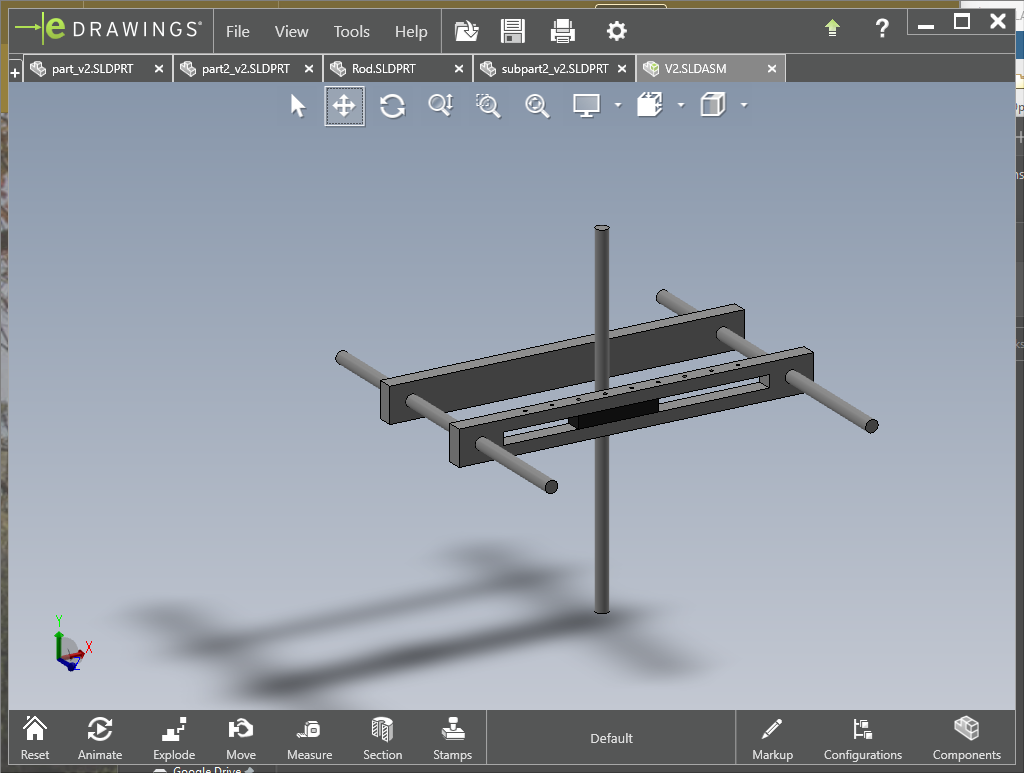
\includegraphics[width=0.25\textwidth]{Main/Ch1/Sample_holder.png}
    \caption{\raggedright 3D Rendering of the sample holder}
    \vspace{.2cm}
\end{wrapfigure}

The sample holder consists of two plastic blocks that are held together by two steel bars. Thumbscrews are used to lock the relative position of the plastic pieces in place while the assembly 'floats'  on the lip of the beaker the sample is submerged into. One of the two plastic pieces has a stopper that helps constrain the position of the assembly on the beaker while the other plastic piece holds the glass rod and alligator clip.

The glass rod is attached to the plastic piece and has the alligator clip on it. The clip and corresponding cathode holder are wrapped in a PTFE sleeve that helps minimize stray electric fields and electroplating onto the cathode wire.


\begin{wrapfigure}{R}{0.35\textwidth}
    \centering
    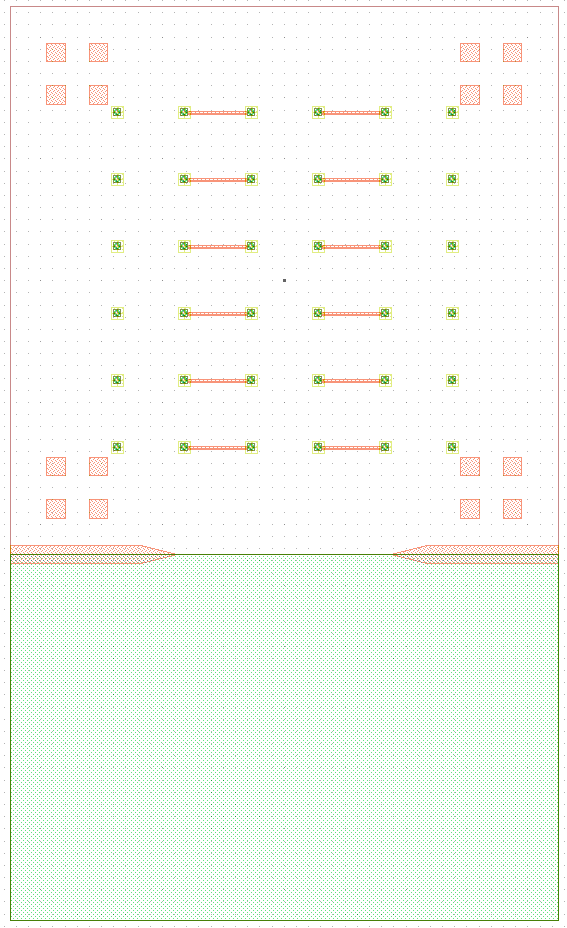
\includegraphics[width=0.35\textwidth]{Main/Ch1/GDS_V1.png}
    \caption{GDS image of the layout. Indium is in green bumps have a diameter of 40 $\um$}
    \label{fig:gds_ch1}
    \vspace{.2cm}
\end{wrapfigure}


\subsection{Physical Problems with the setup}

% TODO Replace derivative with derivative library maybe?
The existing setup came with an analog voltage supply that was only able to provide analog control of the voltage based on two knobs (a fine and coarse). This control was only fine enough to $\pm 10 \mV$ where the derivative of the current with respect to voltage in the relevant regime was $\frac{d \mA}{d \mV} = \frac{0.3 \mA}{1 \mV}$.
This meant there was poor resolution on the current control with the previous power-supply with a current resolution of $\pm 3 \mA$ which would be an insufficient resolution for the small area that was being plated.

I replaced the existing voltage supply with a Tektronics function generator as it provided an appropriate resolution and dynamic range for such the task.
The function generator would allow for pulsed plating as recommended by the indium corporation \cite{indiumCorpGrainStructure}

\newpage
\subsection{Experimental Issues - Deviation from Theory}

According to the Indium corporation docs, the recommended electroplating current density for plating is $10-100 \jufeet$ at $20 \jufeet$ we should observe plating growth at $1.5 \mmph$.
Converting to SI units from ASME units we see that this yields a plating current of $ J_{Plating} \approx 0.11-1.1 \junits \rightarrow I_{Plating} = 2.907 \mA$. However, in this analysis we have only considered the active plating area of the sample, and we have failed to consider the plating area of the exposed alligator clip that holds the sample.

The extra exposed area guarantees an incorrect characterization of the plating growth proportional to the exposed area for the indium bumps. We can show this simply from the following

\begin{equation}\tag{A}
    \begin{split}
        V &\doteq I R \\
        I_{Plating} &\doteq J_{Plating} \times A_{Plating} \\
        R_{Total} &\doteq R_{Anode} + R_{Plating Solution} + R_{Cathode} + R_{Wires} \\
        V_{Plating} &\doteq \text{Variable to satisfy plating current}
    \end{split}
\end{equation}

From the datasheets from Indium Corporation \cite{indiumCorpPlating} we see that the recommended plating current density.

\begin{figure}[t]
    \centering
    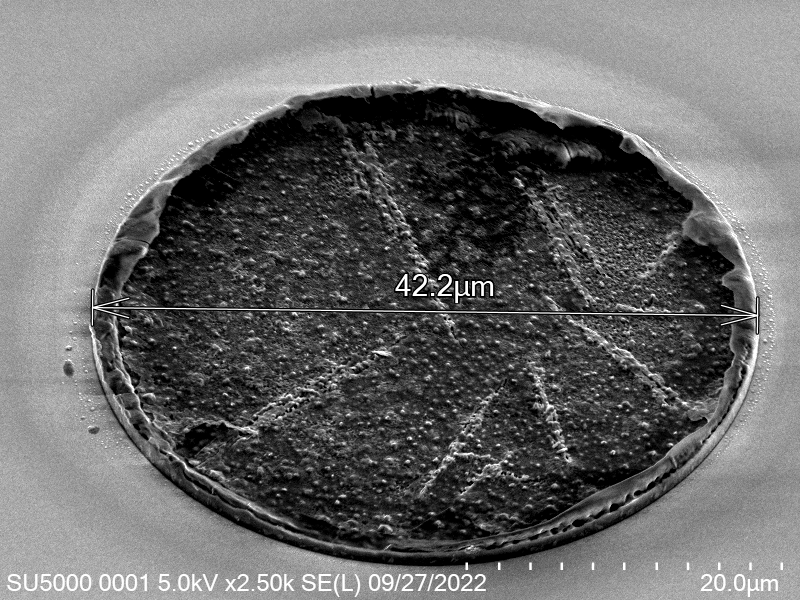
\includegraphics[width=0.48\textwidth]{Main/Ch1/24mA_Growth1.png}
    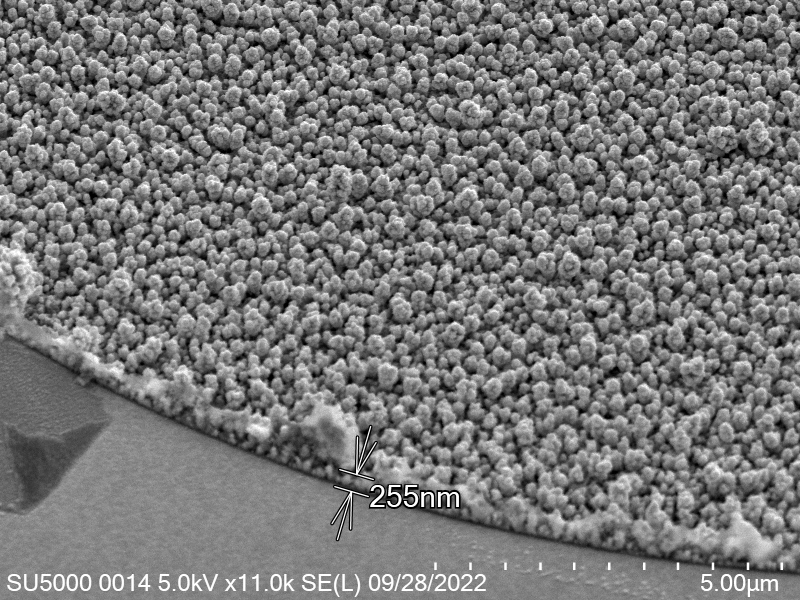
\includegraphics[width=0.48\textwidth]{Main/Ch1/24mA_Growth2.png}
    \caption{\raggedright SEM images of indium bumps for $2.4 \mA$ current for $5 \unit{\min}$}
    \vspace{.2cm}
    \label{fig:24mAGrowth}
\end{figure}


$$
    J_{Plating} = 10-100 \jufeet
$$

Or in more elegant units:

\begin{equation}\notag
    \begin{split}
        J_{Plating} &\approx 0.11-1.1 \junits
    \end{split}
\end{equation}


We can then solve for the plating current based on the exposed area given by the GDS file of the sample in figure \ref{fig:gds_ch1}.


The exposed area is thus:

\begin{equation}\notag
    \begin{split}
        A_{Plating} &= \pi (20 \um)^2 + (4.5 \mm \times 3 \mm) \\
        &\approx 13.5 \sqmm
    \end{split}
\end{equation}

Thus, the plating current for a current density of $20\jufeet$ or $0.2153 \junits$ which represents a growth rate of $1.5\mmph $ or $25 \umpm$ is as follows.

\begin{equation}\notag
    \begin{split}
        I_{Plating} &\doteq J_{Plating} \times A_{Plating} \\
        I_{Plating} &= (0.2153 \junits) \times (13.5 \sqmm) \\
        I_{Plating} &= 2.907 \mA
    \end{split}
\end{equation}


However, when we apply a voltage of $2.4 \mA$ for 5 minutes the growth we see in figure \ref{fig:24mAGrowth} that the growth is between $0.3-1.2 \um$ in thickness.


From those results we can see that the estimate of area that we predicted we got $\frac{0.8}{25} \times 100\% = 3.2\%$ of the expected growth. While that is not explicitly a problem, the indium bumps and growth did not look very uniform or nearly thick enough compared to what would be needed in the proceeding steps.

From here a number of more experiments were conducted and condensed results of the growth were compiled in the table \ref{table:platingGrowths}


\begin{sidewaystable}
    \centering
    \begin{tabular}{| l | l | l | l | l |}
        \hline
        Sample Name & Electroplating Time ($\unit{\min}$)  & Electroplating Current ($\mA$) & Indium Thickness ($\um$) & Growth rate ($\unit{\micro\meter\per\min}$) \\
        \hline
        \hline
        01-Caesar       &    5   &   2.4   &   1.1   &   0.22       \\
        02-Augustus     &    5   &   2.4   &   0.4   &   0.08       \\
        03-Tiberius     &    10  &   2.4   &   1.3   &   0.13       \\
        04-Caligula     &    5   &   4.8   &   1     &   0.2        \\
        05-Claudius     &    10  &   4.8   &   1.3   &   0.13       \\
        06-Nero         &    10  &   9.6   &   1.7   &   0.17       \\
        07-Galba        &    5   &   50    &   5     &   1          \\
        08-Otho         &    5   &   100   &   14    &   2.8        \\
        09-Vitellius    &    5   &   20    &   8.4   &   1.68       \\
        10-Vespasian    &    5   &   30    &   8.3   &   1.66       \\
        11-Titus        &    5   &   40    &   8.5   &   1.7        \\
        12-Domitian     &    5   &   60    &   10    &   2          \\
        13-Nerva        &    5   &   20    &   7.6   &   1.52       \\
        14-Trajan       &    5   &   20    &   5.6   &   1.12       \\
        15-Hadrian      &    5   &   20    &   4     &   0.8        \\
        16-Pius         &    5   &   20    &   4     &   0.8 \\
        \hline
        \hline
    \end{tabular}
    \caption{Table of condensed results of Phase 1 plating experiments}
    \label{table:platingGrowths}
\end{sidewaystable}


\begin{figure}
    \centering
    \begin{tikzpicture}
        \begin{axis}[
            xlabel=Electroplating Current ($\mA$),
            ylabel=Growth rate ($\unit{\micro\meter\per\min}$),
            grid = both,
            % xmode=log,
            ymode=log,
            minor tick num = 1,
            major grid style = {lightgray},
            minor grid style = {lightgray!25},
            legend pos=north west
        ]
        \addplot[
            purple1,
            only marks
        ] table[
            x=x,
            y=y
        ] {Main/Ch1/data.dat};
        % Linear regression
        \addplot[
            thick,
            dotted,
            purple4
        ] table[
            x=x,
            y={create col/linear regression={y=y}}
        ] {Main/Ch1/data.dat};
        \addplot[
            domain=0:100,
            samples=200,
            purple3
        ] {25*x};
        \addlegendentry{Data}
        \addlegendentry{
            Linear regression: $ y =
            \pgfmathprintnumber{\pgfplotstableregressiona}
            \cdot x
            \pgfmathprintnumber[print sign]{\pgfplotstableregressionb}$
        };
        \addlegendentry{Ideal Plating Rate}

        \end{axis}
    \end{tikzpicture}
    \caption{A scatter plot of current vs growth rate.}
    \label{fig:scatterplot}
\end{figure}



\subsection{Development of a Repeatable Process}
In summary, the highlighted issues here have to do with the excessive easy by which the sample holder assembly floats on the beaker, this can in instances cause significant change in the plating rate as seen by the large variance in plating rate as seen in the scatter plot figure \ref{fig:scatterplot}. I must ensure that the sample is well aligned and distanced appropriately from the indium anode to minimize confounding factors.

Secondly in this section we improved plating current control with the use of a digital function generator and an ammeter in series. With this control of the plating current density was significantly improved by almost 1 order of magnitude.

